\chapter{Requirement specification}
\label{kravsspec}
In the following chapter a simple requirement specification for the \textit{FingerDrums} will be presented. A Use Case diagram will also be presented in order to explain how the system should act.

%
I dette kapitel opstilles en projektplan med en generel produktbeskrivelse og specifikke systemkrav. Projektplanen, produktbeskrivelsen og systemkravene formuleres for at produktet i sidste ende kommer til at fungere efter hensigten. Produktet beskrives først generelt ved hjælp af Use Cases. På baggrund af den generelle produktbeskrivelse formuleres en række specifikke systemkrav. De endelige krav vil til sidst opsummeres i prioriteret rækkefølge. 

\section{General description}
%Målet for projektet er at udarbejder et elektronisk instrument, som kan simulere lyde fra et trommesæt. De forskellige trommelyde afspilles ved hjælp af fingerspidserne, hvor hver fingerspids har sin egen unikke lyd. En lyd afspilles når en finger laver en trommebevægelse. En trommebevægelse er en gestikulering hvor fingerspidsen rammer en overflade og derved møder modstand. Modstanden detekteres af en elektronisk sensor. En trommebevægelse kan derved laves på mange forskellige overflader, eksempelvist et bord, en væg eller et lårben. Brugeren af produktet vælger med fingerspidsernes sensorer hvilken lyd der skal afspilles og hvornår den skal afspilles.
%
%Trommelydende kan i princippet varieres og skiftet ud efter brugerens ønske. Som udgangspunkt kan en unik lyd for hver fingerspids frembringes. Brugeren kan ved hjælp af et display udskifte eller omarrangere de unikke lyde efter behov. På den måde kan produktet tilpasses specifikke brugere samt brugssituationer. Brugeren kan ændre lydstyrken ved hjælp af displayet. Det er også ved hjælp af displayet at produktets tænd/sluk funktion tilgås. 

The \textit{FingerDrums} is integrated in a glove which helps to hold the sensors in place. Ideally the user has an interface to be able to change the sound profile and volume around the wrist and opening of the glove. For this prototype the sensors are wired to an Arduino which communicates with the PC. The PC then plays the sounds. No interface is integrated on the wrist in this iteration.

\section{Use Cases}
Here the basic functional requirements will be listed in a Use Case diagram which explains the actors on the system and how they are correlated between each other.
%Følgende afsnit fokusere på de funktionelle krav som produktet skal opfylde. Produktets funktioner beskrives ved hjælp af Use Cases, hvor grænseflader mellem aktører og funktioner vil fremgå. Den generelle produktbeskrivelse lægger op til uddybelse af produktets funktionelle krav, samt en opdeling af de aktører, som indgår i processen.
In order for the \textit{FingerDrums} concept to work the user should be able to play sounds, determine which sounds should be played, change the volume and turn the system on/off. As mentioned at the top in \autoref{Ideation} the purpose is to develop an electrical prototype which allows to play drum sounds and perhaps contain a display. On \autoref{fig:protoUseCase} the Use Case diagram is shown. The internal actors are denoted Display, Sensors, and Control System. 

Brugeren af produktet skal have mulighed for at afspille lyde, udskifte lyde, ændre lydstyrke samt tænde og slukke for systemet. Afspil lyd, Udskift lyd, Ændr lydstyrke og Tænd/sluk er derfor essentielle funktioner at implementere, for at produktet fungere optimalt. For at brugeren i sidste ende kan tilgå funktionerne er det nødvendigt at kende de interne og eksterne aktører som er involveret i  processerne. Som nævnt i ***section - Generel produktbeskrivelse*** er målet for projektet at fremstille en elektronisk prototype, som ved hjælp af et styresystem kan afspille forskellige trommelyde på baggrund af brugerens interaktion med sensorer og et display. De interne aktører; Sensorer, Display og Styresystem, symboliserer hvor der foregår en interaktion mellem produktets forskellige funktioner og aktører. Brugeren selv defineres som en ekstern aktør, ligsom højtaler, der i sidste ende afspiller lyden, også fremgår som eksterne aktører. Det sker for at simplificere Use Case diagrammet til kun at omfatte systemet selv. Use Case diagrammet på \autoref{fig:protoUseCase} fokusere derfor på de interne aktører, som gør funktionerne tilgængelige via grænsefladerne mellem funktion og aktør. 

\begin{figure}
\centering
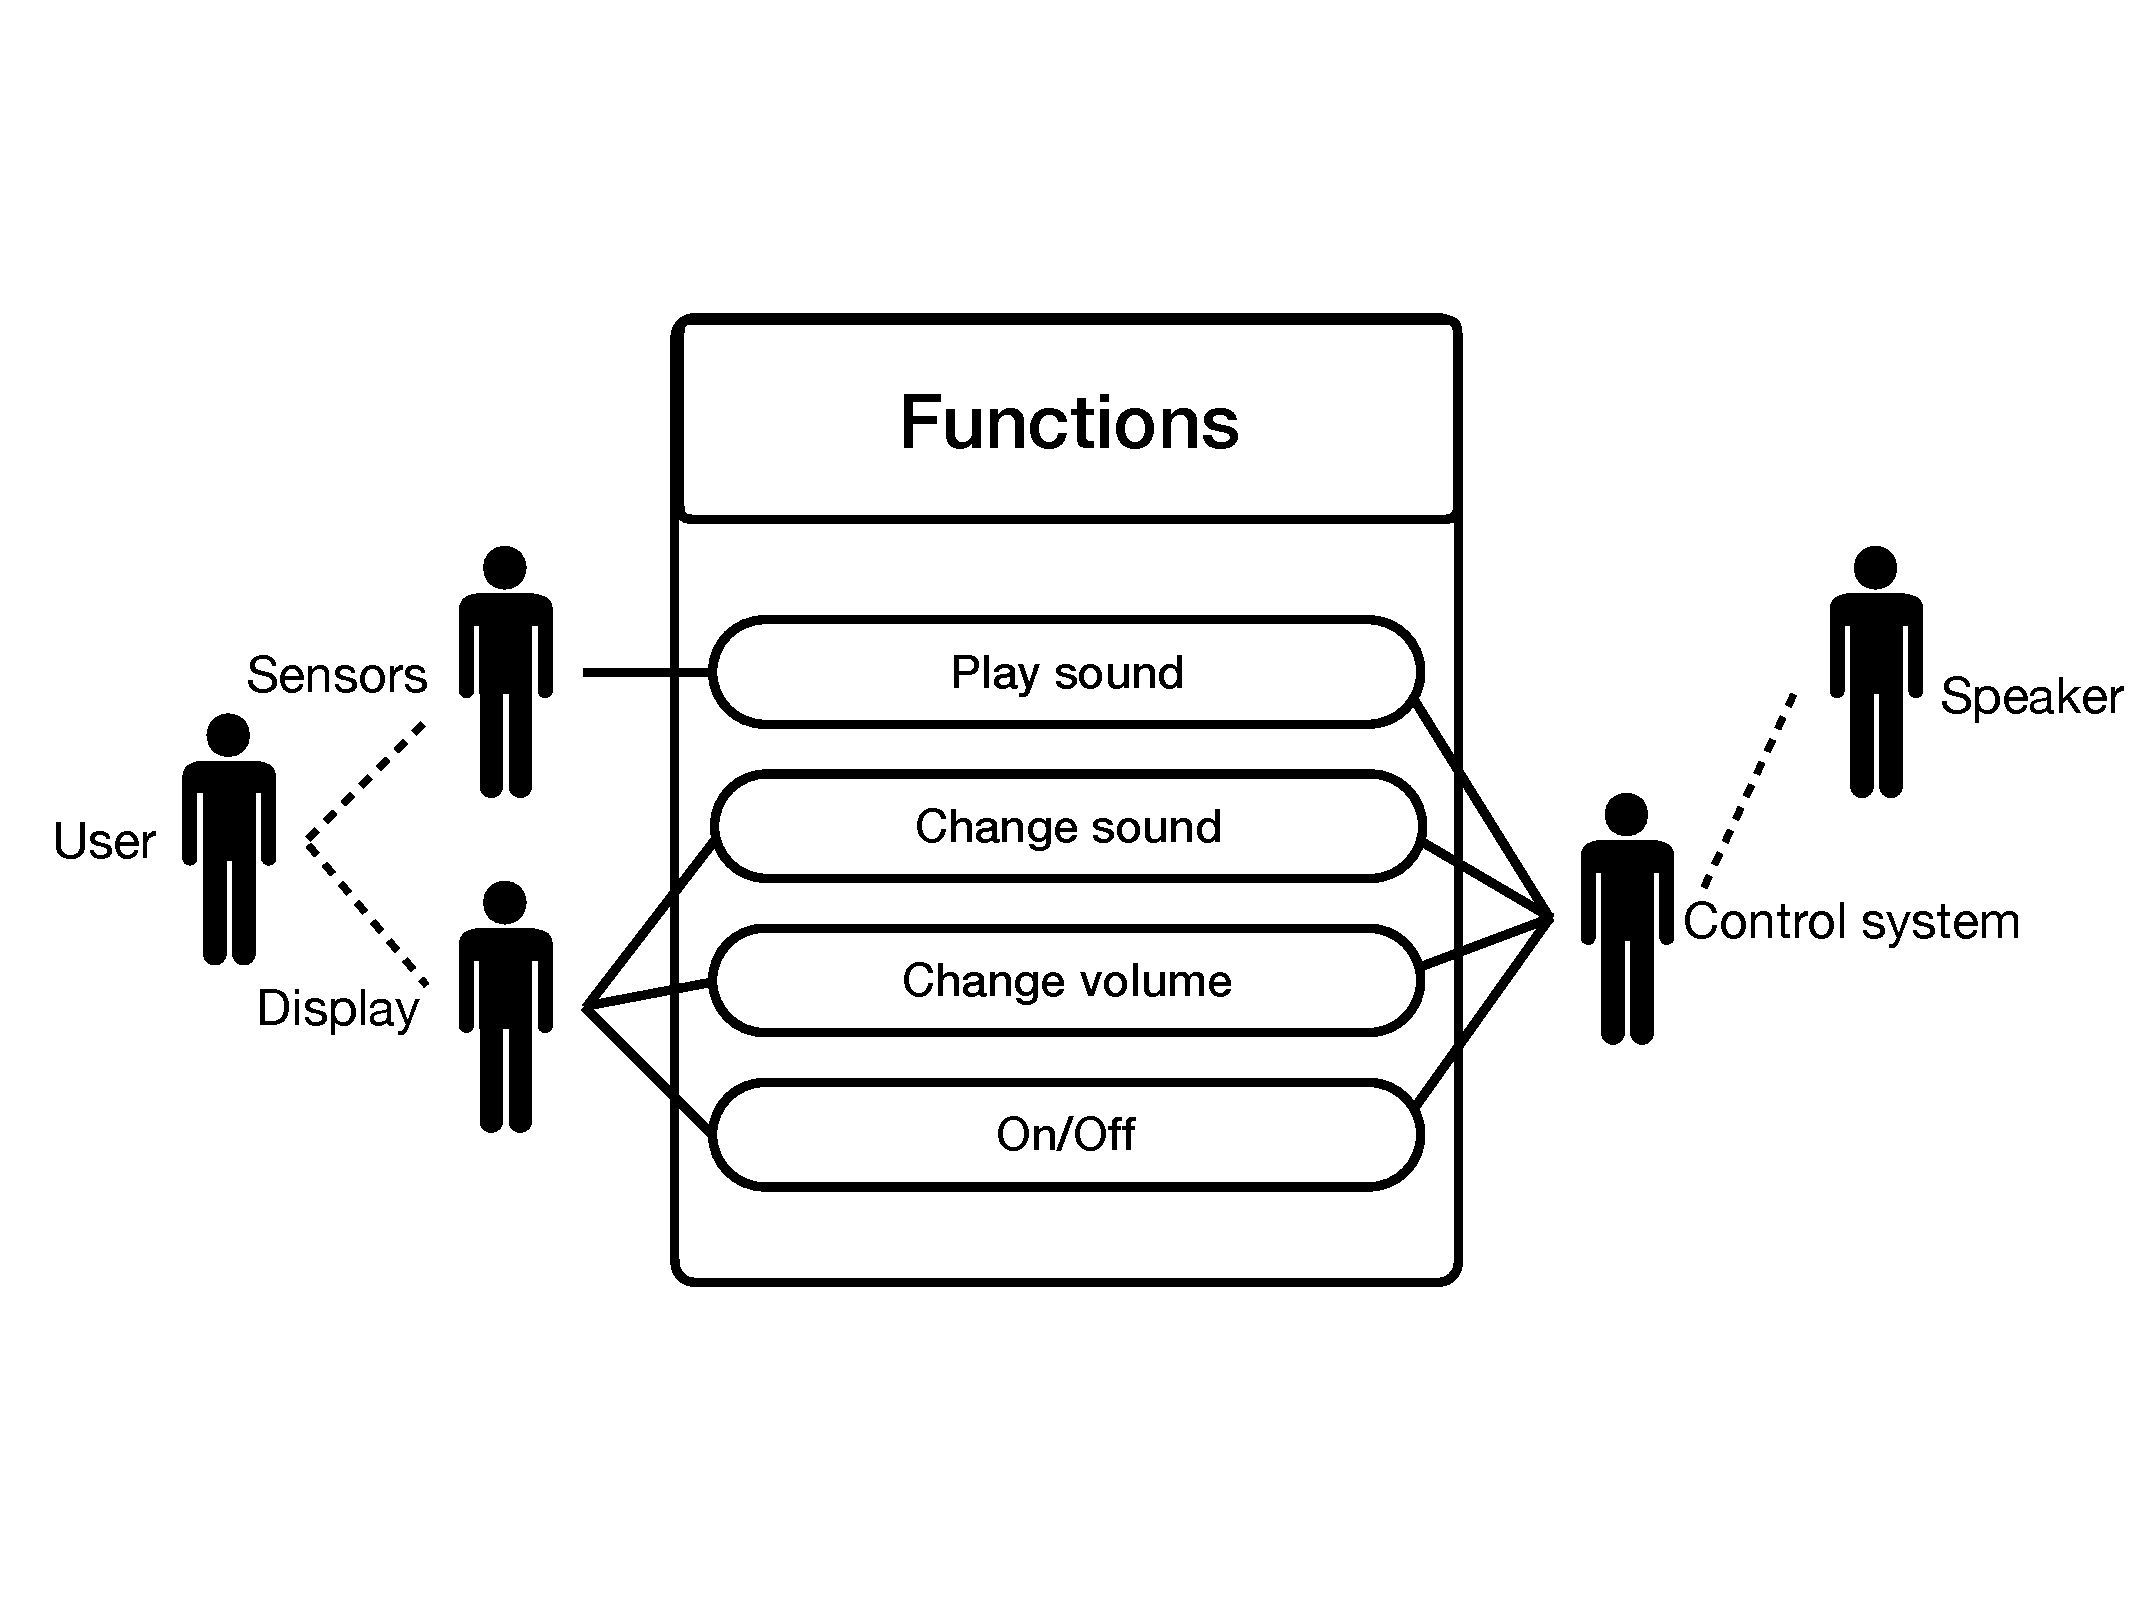
\includegraphics[scale=0.4]{Figure/protoUseCase01.pdf}
\caption{
Use Case diagram for det samlede system. De fire Use Cases er forbundet til deres respektive aktører. Mellem Use Case og aktør findes grænsefladen, som er udtryk for hvilke aktører der kommunikere med hinanden.}
\label{fig:protoUseCase}
\end{figure}

\subsection{Afspil lyd}
Brugeren interagere med sensorerne for at afspille en unik trommelyd. Sensorerne signalere, via grænsefladen til styresystemet, at en finger laver en trommebevægelse. Styresystemet reagere på signalet og interagere med den eksterne aktør, højtaler, der derefter afspiller lyden.    

\subsection{Udskift lyd}
Brugeren interagere med displayet for at udskifte eller omarrangere en lyd. Displayet signalere, via grænsefladen til styresystemet, at en lyd skal ændres. Styresystemet reagere på signalet og ændre derefter den respektive lyd.   

\subsection{Ændr lydstyrke}
Brugeren interagere med displayet for at ændre lydstyrken. Displayet signalere, via grænsefladen til styresystemet, at lydstyrken skal ændres. Styresystemet reagere på signalet og ændre derefter lydstyrken. 

\subsection{Tænd/sluk}
Brugeren interagere med displayet for at tænde eller slukke systemet. Displayet signalere, via grænsefladen til styresystemet, at systemet enten skal tændes eller slukkes. Styresystemet reagere på signalet, hvorefter systemet enten tænder eller slukker

\section{Specifikke krav}
Følgende afsnit giver en detaljeret beskrivelse af de specifikke krav der måtte være til produktet. Først beskrives kravende til funktionaliteten, derefter kravende til de interne aktører og til sidst beskrives kravende til det samlede system, herunder kvalitetskrav og designkrav. 

\subsection{Krav til funktionalitet}
\label{Krav_til_funktionalitet}

Som det fremgår af afsnit ***HENVISNING ÚSE CASES***, skal fire funktioner implementeres. Funktionerne initieres via aktørerne Sensor og Display. Aktørerne virker som brugerinterface, og er dermed brugerens mulighed for at interagere med aktøren Styresystem. Selve funktionerne eksekveres af aktøren Styresystem.

Ved funktionen, Afspil lyd, menes muligheden for at afspille en specifik lydfil ækvivalent til den sensor brugeren interagere med. Lydfilen skal som udgangspunkt imitere en lyd fra et trommesæt. Lyden forventes derfor at bestå af et kompleks signal frem for en ren sinustone. Lyden afspilles umiddelbart efter brugeren har interageret med en sensor, uden mærkbar forsinkelse. En mærkbar forsinkelse defineres som en forsinkelse hvor auditive feedback afspilles tilpas lang tid efter interaktionen med sensoren til at brugeren kan detektere en forsinkelse. Lyden afspilles en enkelt gang ved hver interaktion med en sensor. Hvis brugeren interagere med flere sensorer samtidigt afspilles de respektive lyde samtidig.  

Ved funktionen, Udskift lyd, menes muligheden for at udskifte de specifikke trommelyde. Derved har brugeren mulighed for at udskifter og omarrangere de lyde der frembringes ved at intergere med en sensor. Lydene udskiftes ved at interagere med aktøren display, hvorefter styresystemet ændre de respektive lyde. 

Ved funktionen, Ændr lydstyrke, menes muligheden for at skrue op og ned for lydstyrken af trommelydene. Derved kan brugeren dimensionere lydniveauet så det passe til omgivelserne. Lydstyrken ændres ved at interagere med aktøren display, hvorefter styresystemet ændre lydstyrken.

Ved funktionen, Tænd/Sluk, menes muligheden for at tænde eller slukke for systemet. Derved har brugeren mulighed at vælge hvornår systemet er aktivt og afspiller lyde ved interaktion med sensorerne.

\begin{enumerate}
\item[\textbf{§}] \textbf{1} Afspil lyd \fxnote{der skal en mere specifik beskrivelse til. etc. afspil lyd fra hvad? igennem hvad?}
\item[\textbf{§}] \textbf{2} Udskift lyd
\item[\textbf{§}] \textbf{3} Ændr lydstyrke
\item[\textbf{§}] \textbf{4} Tænd/Sluk
\end{enumerate}
\subsection{Krav til aktører}
\subsection{krav til samlet system}


 


-----------------------------

Hovedfunktioner: 
Begrænsninger:
Brugerprofiler:

Specifikke krav: 
Sensorene skal kunne signalere om en respektiv finger trommer eller ej. 
Styringsenheden skal kunne aflæse signalet fra sensorerne, behandler signalet og afspille en lydfil til en højtaler.

… detailkrav/
ydelseskrav/
kvalitetskrav/
designkrav/ - flexibel let handske      

 
